\documentclass[11pt,a4paper]{article}

% --- Préambule (Conservé de votre modèle) ---
\usepackage[utf8]{inputenc}
\usepackage[T1]{fontenc}
\usepackage[french]{babel}
\usepackage[margin=2.5cm]{geometry}
\usepackage{amsmath, amssymb}
\usepackage{graphicx}
\usepackage{xcolor}
\usepackage{parskip}
\usepackage{titlesec}
\usepackage{siunitx}
\usepackage{booktabs}
\usepackage{pgfplots}
\pgfplotsset{compat=1.18}
\usepackage{float}
\usepackage{hyperref}

% Configuration des liens et couleurs
\hypersetup{
    colorlinks=true,
    linkcolor=blue!70!black,
    urlcolor=blue!70!black,
    pdftitle={Rapport de Laboratoire - Analyse et Régulation d'un Système du Second Ordre}
}
\definecolor{MarineBlue}{HTML}{1A446C}

% Personnalisation des titres de sections
\titleformat{\section}{\Large\bfseries\color{blue!60!black}}{\thesection.}{1em}{}
\titleformat{\subsection}{\large\bfseries\color{black!80}}{\thesubsection.}{1em}{}

\begin{document}

% --- Page de garde personnalisée ---
\begin{titlepage}
    \centering
    \vspace*{3cm}
    
    {\Large \textsc{Cours d'Automatique et Robotique}\par}
    \vspace{2cm}
    
    \rule{\linewidth}{0.5mm} \\[0.4cm]
    {\huge\bfseries Rapport de Laboratoire\\[0.4cm]
    \Large Fonction de transfert}
    \rule{\linewidth}{0.5mm} \\[2.5cm]
    
    {\Large \textbf{Enseignant :} Beco Thomas\par}
    \vspace{3cm}
    
    {\large \textbf{Réalisé par :}\par}
    \vspace{0.5cm}
    {\Large Winant Guilaume\par}
    
    \vfill
    {\large le 27 mai 2026}
\end{titlepage}

\setcounter{page}{1}

% --- Table des matières ---
\tableofcontents
\newpage

% --- Section 1 : Introduction ---
\section{Introduction}

Ce laboratoire est dédié à l'étude des systèmes dynamiques continus linéaires à travers l'outil de programmation Python. L'analyse se concentre sur une fonction de transfert générique du second ordre, un comportement classique et fondamental en ingénierie de contrôle-commande. 

De manière spécifique, les objectifs de ce travail consistent à :
\begin{itemize}
    \item Identifier et analyser les caractéristiques intrinsèques d'un système sous-amorti en boucle ouverte (pulsation propre, coefficient d'amortissement, gain statique) ;
    \item Évaluer le comportement temporel (réponses indicielle et impulsionnelle) et fréquentiel (diagramme de Bode) du procédé ;
    \item Étudier l'influence d'une régulation proportionnelle sur la stabilité globale en confrontant l'approche algébrique du critère de Routh à l'approche fréquentielle graphique de Nyquist et au lieu des racines ;
    \item Concevoir et dimensionner un correcteur Proportionnel-Intégral-Dérivé (PID) par une méthode théorique de placement de pôles afin de satisfaire un cahier des charges de performance prédéfini.
\end{itemize}

% --- Section 2 : Description du matériel ---
\section{Description du matériel}

Les simulations, l'acquisition des données fréquentielles et les synthèses de lois de commande ont été entièrement réalisées de manière logicielle. L'environnement technique comprend :
\begin{itemize}
    \item \textbf{Langage de programmation :} Python 3.10.
    \item \textbf{Bibliothèque d'Automatique (\texttt{control}) :} Utilisée pour la manipulation des fonctions de transfert, le calcul des réponses temporelles (\texttt{step\_response}, \texttt{impulse\_response}), le tracé des diagrammes fréquentiels (\texttt{bode\_plot}) et le lieu des racines (\texttt{root\_locus}).
    \item \textbf{Bibliothèques scientifiques (\texttt{numpy} \& \texttt{math}) :} Utilisées pour la discrétisation vectorielle des plages fréquentielles et temporelles ainsi que pour la formulation des modèles mathématiques analytiques.
    \item \textbf{Bibliothèque graphique (\texttt{matplotlib.pyplot}) :} Employée pour générer des fenêtres d'affichage claires, normées et exploitables au sein de ce rapport.
\end{itemize}

% --- Section 3 : Les analyses ---
\section{Les analyses}

Cette section détaille les fondements mathématiques sous-jacents aux calculs numériques effectués par le script de simulation. La fonction de transfert étudiée s'exprime sous la forme :
\begin{equation}
    H(s) = \frac{2}{3s^2 + s + 1}
    \label{eq:FT_initiale}
\end{equation}

\subsection{Identification des paramètres canoniques}
La forme standard d'un système du second ordre est définie par l'équation suivante :
\begin{equation}
    H(s) = \frac{K_{stat}}{\frac{1}{\omega_n^2}s^2 + \frac{2\zeta}{\omega_n}s + 1}
\end{equation}
Par identification directe avec l'équation \eqref{eq:FT_initiale}, nous établissons le système d'équations permettant d'extraire de manière générique le gain statique $K_{stat}$, la pulsation propre non amortie $\omega_n$, et le coefficient d'amortissement $\zeta$ :
\begin{equation}
    K_{stat} = 2, \quad \omega_n = \sqrt{\frac{1}{3}} \approx \SI{0.5774}{\text{rad/s}}, \quad \zeta = \frac{1}{2\sqrt{3}} \approx 0.2887
\end{equation}

\subsection{Analyse fréquentielle analytique}
La réponse harmonique est obtenue en substituant la variable de Laplace par l'opérateur imaginaire pur $s = j\omega$. L'expression complexe devient :
\begin{equation}
    H(j\omega) = \frac{2}{(1 - 3\omega^2) + j\omega}
\end{equation}
L'amplitude absolue $|H(j\omega)|$ (exprimée ensuite en décibels par $20\log_{10}|H(j\omega)|$) et la phase $\theta(\omega)$ sont déterminées analytiquement par :
\begin{equation}
    |H(j\omega)| = \frac{2}{\sqrt{(1 - 3\omega^2)^2 + \omega^2}}, \quad \theta(\omega) = -\arctan2(\omega, 1 - 3\omega^2)
\end{equation}

\subsection{Étude de stabilité sous régulation proportionnelle (P)}

Afin de contrôler le système, nous insérons un régulateur de gain pur $K$ en amont de notre procédé, le tout dans une boucle à retour unitaire négatif. La fonction de transfert en Boucle Fermée (BF) se calcule par la formule classique $H_{BF}(s) = \frac{K \cdot H(s)}{1 + K \cdot H(s)}$ :
\begin{equation}
    H_{BF}(s) = \frac{K \cdot \left(\frac{2}{3s^2 + s + 1}\right)}{1 + K \cdot \left(\frac{2}{3s^2 + s + 1}\right)} = \frac{2K}{3s^2 + s + 1 + 2K}
\end{equation}

Pour que ce système en boucle fermée soit stable, il faut que les racines de son dénominateur (l'équation caractéristique) soient toutes à partie réelle strictement négative. L'équation caractéristique est :
\begin{equation}
    3s^2 + s + (1 + 2K) = 0
\end{equation}

Pour éviter de calculer les racines complexes, nous utilisons le critère algébrique de Routh-Hurwitz. Construisons le tableau de Routh associé à ce polynôme :
\begin{equation}
    \begin{array}{c|cc}
    s^2 & 3 & 1+2K \\
    s^1 & 1 & 0 \\
    s^0 & b_1 & 0
    \end{array}
\end{equation}

Le terme $b_1$ se calcule à l'aide du déterminant croisé des deux lignes supérieures :
\begin{equation}
    b_1 = \frac{1 \cdot (1+2K) - 3 \cdot 0}{1} = 1 + 2K
\end{equation}

Le théorème de Routh stipule que le système est stable si et seulement si tous les coefficients de la première colonne du tableau sont de même signe (ici, strictement positifs, puisque le premier terme est 3). Nous posons donc nos conditions de stabilité :
\begin{itemize}
    \item Ligne $s^2$ : $3 > 0$ (Condition toujours vérifiée)
    \item Ligne $s^1$ : $1 > 0$ (Condition toujours vérifiée)
    \item Ligne $s^0$ : $1 + 2K > 0$
\end{itemize}

En isolant $K$ dans la dernière inéquation, nous trouvons la limite de stabilité du système :
\begin{equation}
    2K > -1 \implies K > -0.5
\end{equation}

\subsection{Synthèse du correcteur PID par placement de pôles}

Le régulateur proportionnel seul a montré ses limites. Pour obtenir un système à la fois rapide, précis et sans erreur statique, nous utilisons un correcteur PID complet. Son équation de base est $C(s) = K_p + \frac{K_i}{s} + K_d s$, ce qu'on peut réécrire sous forme d'une seule fraction :
\begin{equation}
    C(s) = \frac{K_d s^2 + K_p s + K_i}{s}
\end{equation}

\textbf{1. L'équation du système avec PID :} \\
Si l'on place ce correcteur en boucle fermée avec notre système $H(s)$, la nouvelle équation caractéristique (le dénominateur global de la boucle fermée, donné par $1 + C(s)H(s) = 0$) devient :
\begin{equation}
    s(3s^2 + s + 1) + 2(K_d s^2 + K_p s + K_i) = 0
\end{equation}
En développant et en regroupant les termes de même puissance de $s$, nous obtenons un polynôme du troisième ordre :
\begin{equation}
    3s^3 + (1 + 2K_d)s^2 + (1 + 2K_p)s + 2K_i = 0
    \label{eq:pid_reel}
\end{equation}

\textbf{2. Le comportement désiré (Polynôme cible) :} \\
Notre cahier des charges exige que le système final se comporte "bien" : on souhaite un bon amortissement pour éviter les dépassements brusques ($\zeta_d = 0.7$) et une bonne rapidité ($\omega_{nd} = \SI{2}{\text{rad/s}}$). La dynamique principale d'un tel comportement correspond à un dénominateur classique :
\begin{equation}
    s^2 + 2\zeta_d\omega_{nd}s + \omega_{nd}^2 \implies s^2 + 2.8s + 4
\end{equation}
Cependant, notre système régulé \eqref{eq:pid_reel} est du troisième ordre ($s^3$). Pour pouvoir comparer les équations, nous devons rajouter un pôle (une racine) à notre comportement cible. Pour que ce troisième pôle ne ralentisse pas notre système, on le choisit artificiellement très rapide, loin sur la gauche du plan complexe (la règle empirique est de le placer à $10 \times \zeta_d \omega_{nd}$, soit $p_3 = -14$). L'équation de notre polynôme cible parfait est donc :
\begin{equation}
    (s^2 + 2.8s + 4)(s + 14) = s^3 + 16.8s^2 + 43.2s + 56 = 0
\end{equation}
Afin de pouvoir comparer cette équation cible avec notre vraie équation \eqref{eq:pid_reel} qui commence par $3s^3$, nous multiplions tout le polynôme cible par 3 :
\begin{equation}
    3s^3 + 50.4s^2 + 129.6s + 168 = 0
    \label{eq:pid_cible}
\end{equation}

\textbf{3. Identification des paramètres :} \\
Il ne reste plus qu'à forcer notre système réel \eqref{eq:pid_reel} à correspondre parfaitement au comportement idéal \eqref{eq:pid_cible}. Par simple identification membre à membre (coefficient par coefficient), nous déduisons les valeurs de notre PID :
\begin{itemize}
    \item Pour $s^2$ : $1 + 2K_d = 50.4 \implies K_d = 24.7$
    \item Pour $s^1$ : $1 + 2K_p = 129.6 \implies K_p = 64.3$
    \item Pour $s^0$ : $2K_i = 168 \implies K_i = 84$
\end{itemize}
\vspace{0.2cm}
Cette méthode théorique, appelée "placement de pôles", garantit de manière mathématique que le système régulé adoptera la dynamique exacte que nous avons choisie.

\newpage

% --- Section 4 : Les résultats ---
\section{Les résultats}

\subsection{Comportement temporel du système non régulé}
Puisque le coefficient d'amortissement calculé est compris entre 0 et 1 ($\zeta = 0.2887$), le système est qualifié de sous-amorti. Les réponses obtenues sous Python valident parfaitement ce comportement.

\begin{figure}[H]
    \centering
    % Réglage de l'épaisseur du trait et de l'espace (padding)
    \setlength{\fboxrule}{3pt} 
    \setlength{\fboxsep}{3pt} 
    % Création du cadre (Bordure bleue, fond blanc)
    \fcolorbox{MarineBlue}{white}{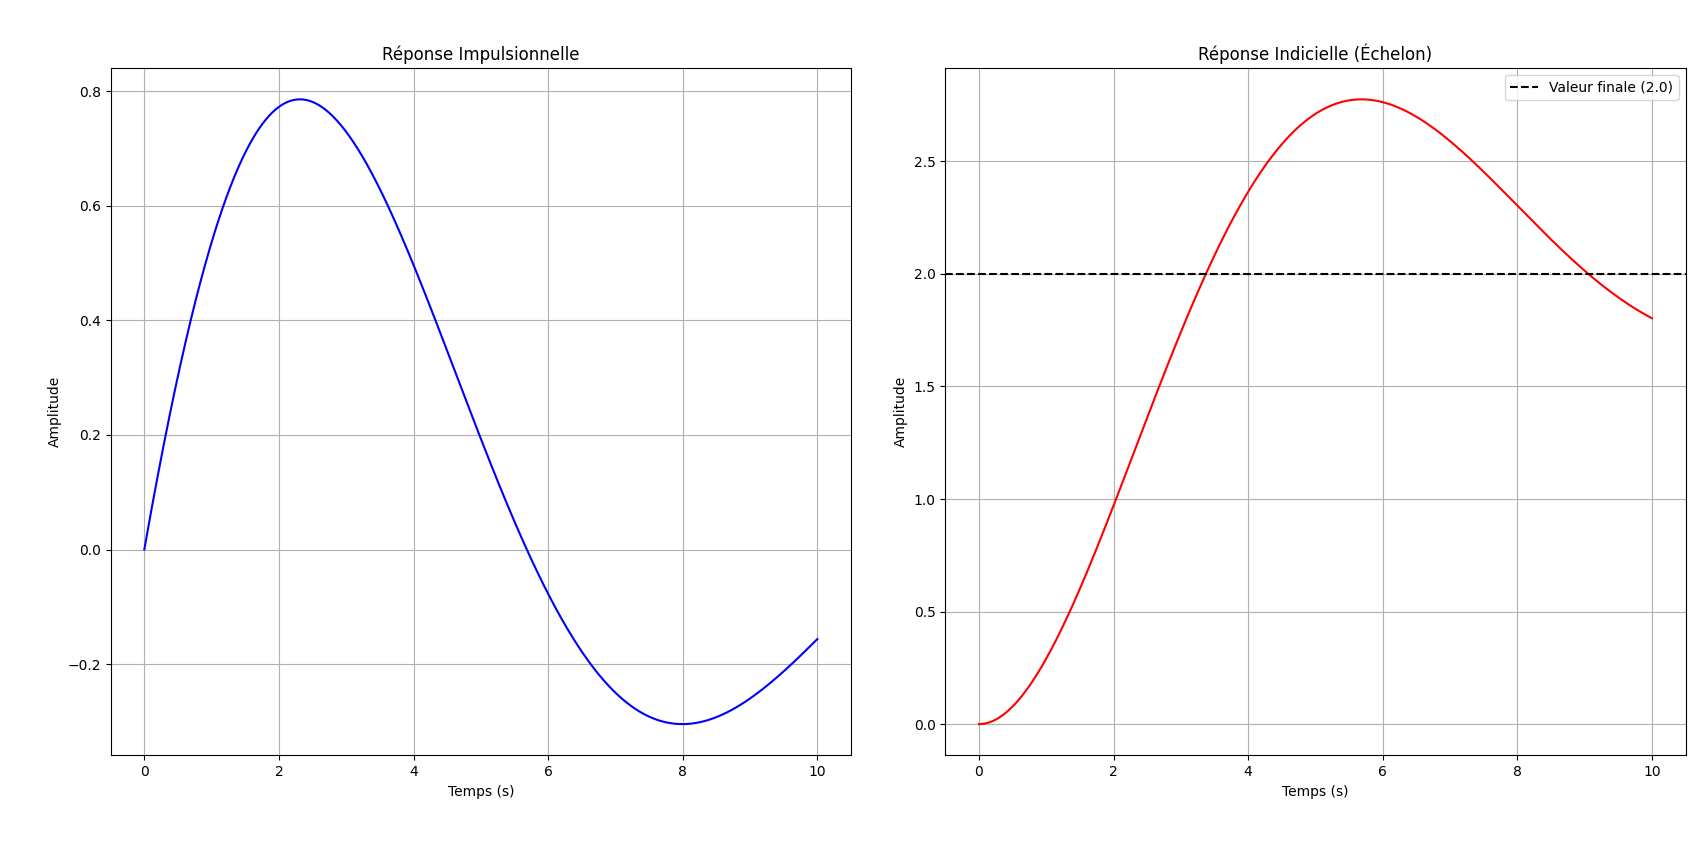
\includegraphics[width=0.8\textwidth]{Figure_1.png}}
    \caption{Évolution temporelle du système du second ordre en boucle ouverte.}
    \label{fig:temporel}
\end{figure}

\textit{Commentaire :} La réponse indicielle confirme un gain statique égal à 2.0. Le faible amortissement engendre un dépassement initial prononcé (proche de 40\%) suivi d'oscillations transitoires avant stabilisation complète en environ \SI{8}{\second}.

\subsection{Validation de l'analyse fréquentielle}
Le diagramme de Bode généré illustre l'atténuation classique de \SI{-40}{\text{dB/décade}} en haute fréquence et un déphasage asymptotique glissant vers \SI{-180}{\degree}.

\begin{figure}[H]
    \centering
    \setlength{\fboxrule}{3pt} 
    \setlength{\fboxsep}{3pt} 
    \fcolorbox{MarineBlue}{white}{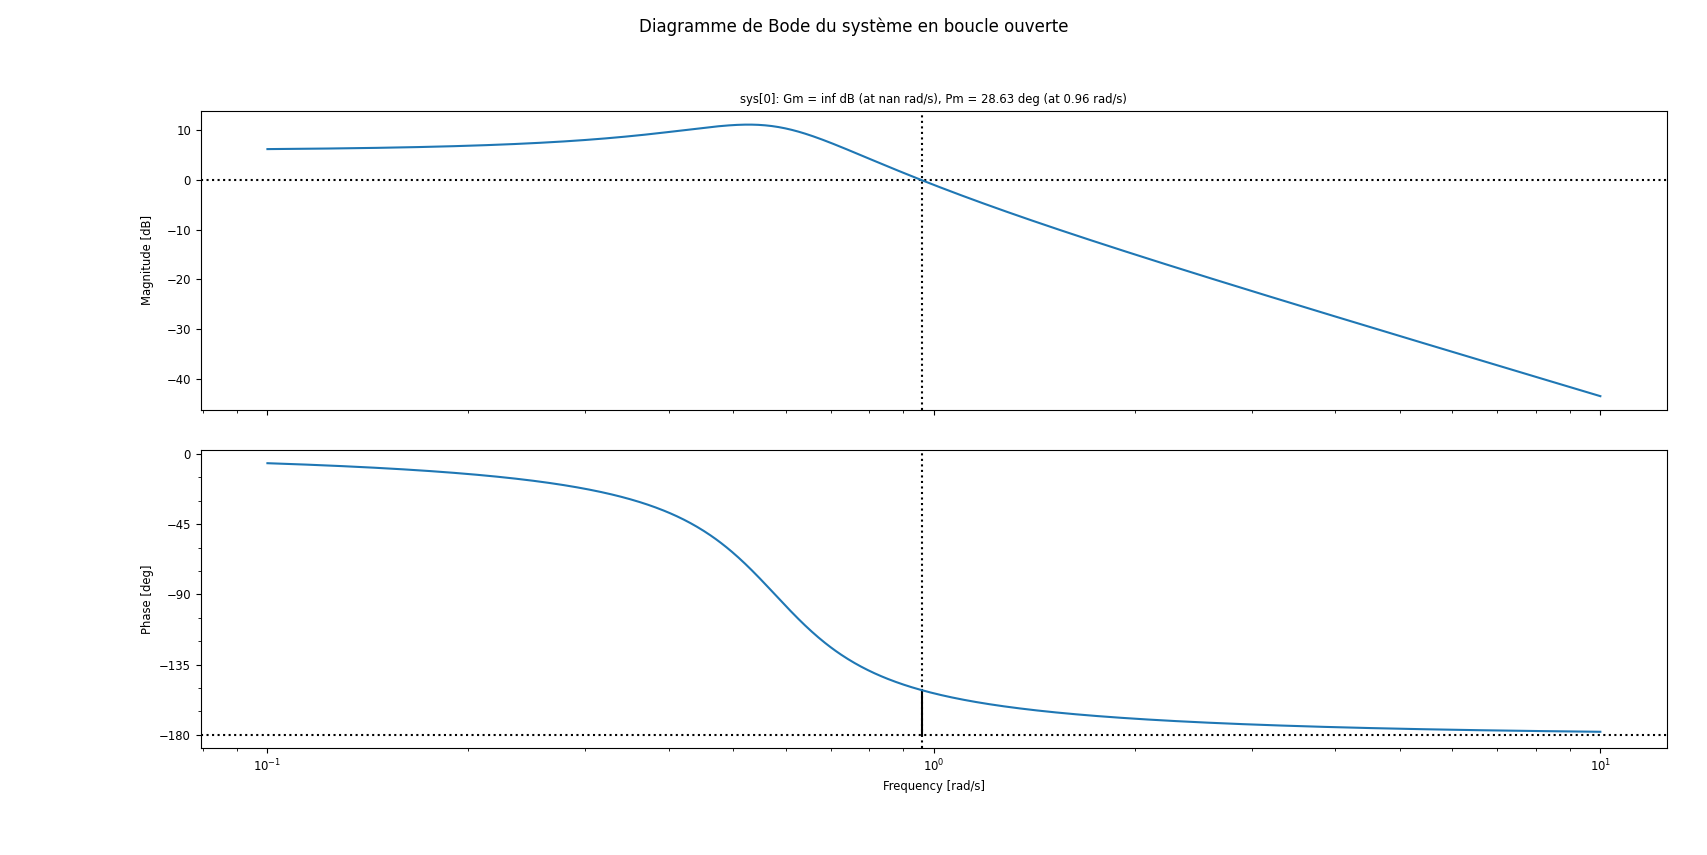
\includegraphics[width=0.7\textwidth]{Figure_2.png}}
    \caption{Diagramme de Bode du système en boucle ouverte.}
    \label{fig:bode}
\end{figure}

Le tableau \ref{tab:frequentiel} met en évidence la stricte concordance entre les points évalués automatiquement via Python et les formulations analytiques développées à la section précédente.

\begin{table}[H]
\centering
\caption{Comparaison des données fréquentielles graphiques et analytiques.}
\label{tab:frequentiel}
\begin{tabular}{lcccc}
\toprule
& \multicolumn{2}{c}{\textbf{Méthode Automatique (Python)}} & \multicolumn{2}{c}{\textbf{Calcul Analytique}} \\
\cmidrule(lr){2-3} \cmidrule(lr){4-5}
\textbf{Pulsation} $\omega$ & \textbf{Gain (dB)} & \textbf{Phase (°)} & \textbf{Gain (dB)} & \textbf{Phase (°)} \\
\midrule
\SI{0.1}{rad/s} & 6.24 & -5.89 & 6.24 & -5.89 \\
\SI{1.0}{rad/s} & -0.97 & -153.43 & -0.97 & -153.43 \\
\SI{10.0}{rad/s} & -43.50 & -178.08 & -43.50 & -178.08 \\
\bottomrule
\end{tabular}
\end{table}

\subsection{Stabilité sous contrôle proportionnel}
Le tracé sur-mesure du critère graphique de Nyquist permet d'observer le comportement du contour vis-à-vis du point critique $(-1, 0)$ pour trois valeurs distinctes de gain $K$.

\begin{figure}[H]
    \centering
    \setlength{\fboxrule}{3pt} 
    \setlength{\fboxsep}{3pt} 
    % On met width=0.95 ou \textwidth car cette image contient 3 graphiques côte à côte
    \fcolorbox{MarineBlue}{white}{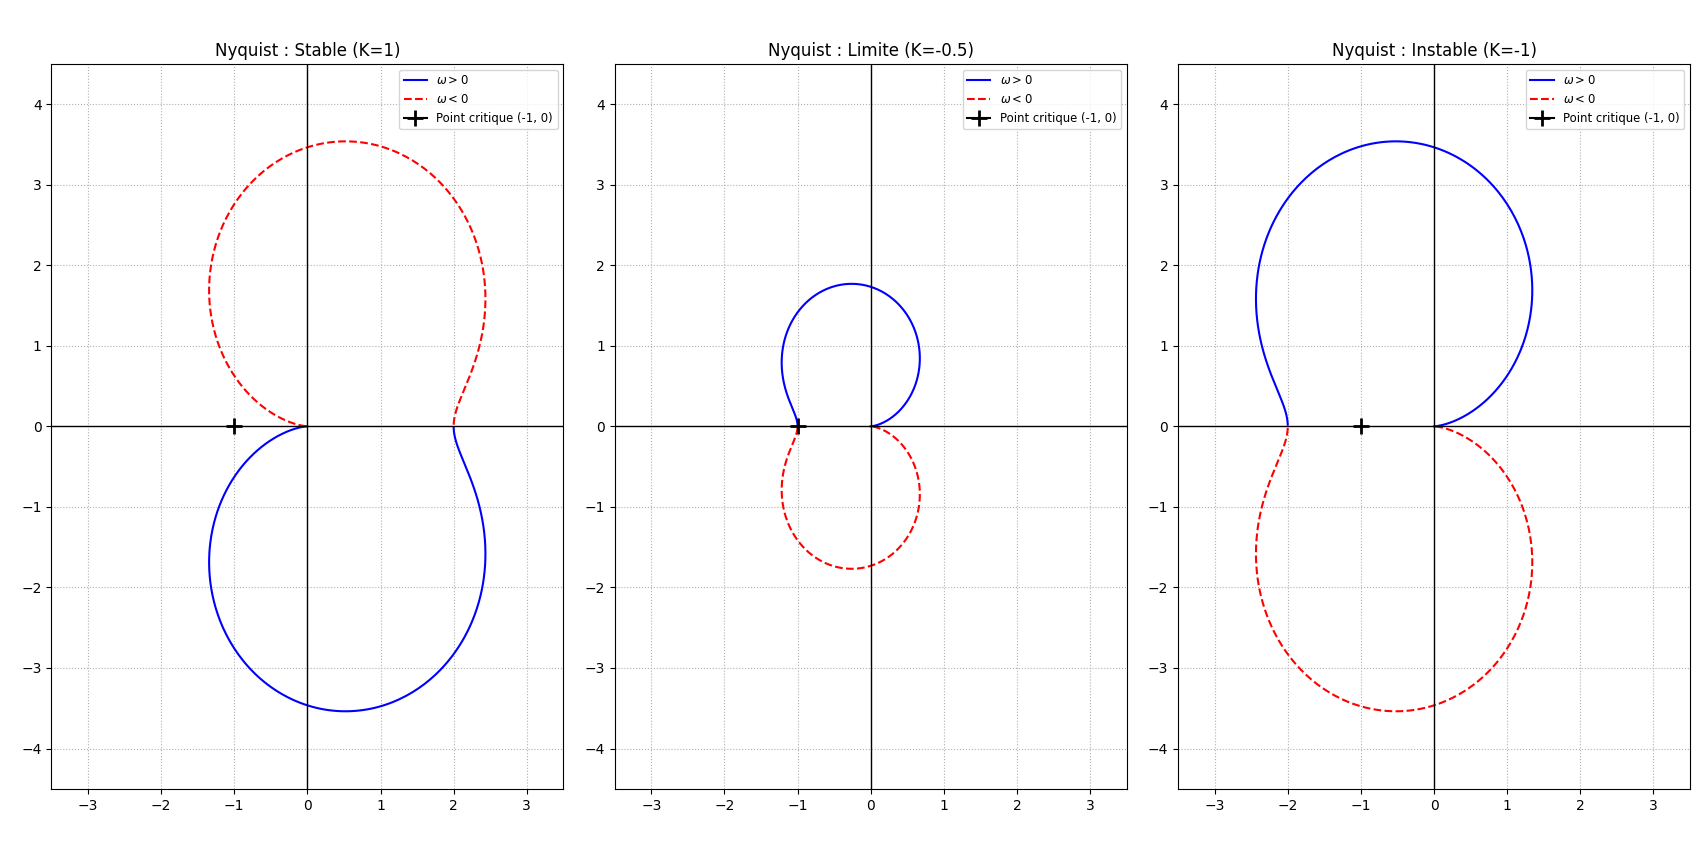
\includegraphics[width=0.8\textwidth]{Figure_3.png}}
    \caption{Lieux de Nyquist et étude du point critique de stabilité.}
    \label{fig:nyquist}
\end{figure}

\begin{figure}[H]
    \centering
    \setlength{\fboxrule}{3pt} 
    \setlength{\fboxsep}{3pt} 
    \fcolorbox{MarineBlue}{white}{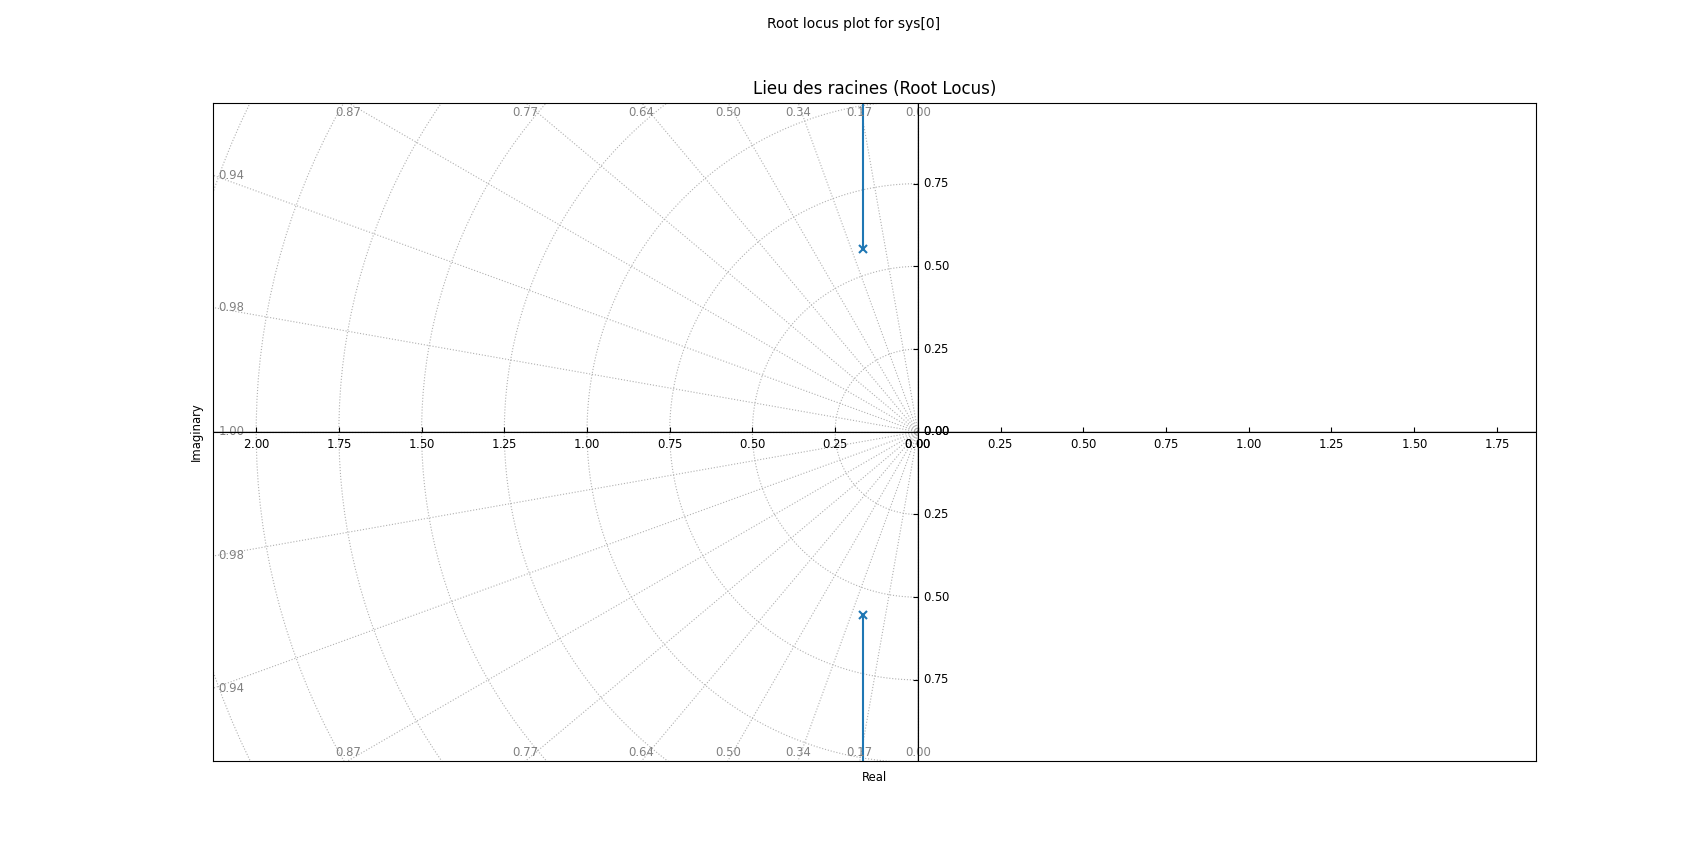
\includegraphics[width=0.8\textwidth]{Figure_4.png}}
    \caption{Lieu des racines du système sous gain variable.}
    \label{fig:root_locus}
\end{figure}

\textit{Analyse de stabilité :} Le graphique de Nyquist pour $K=1$ n'encercle pas le point $(-1,0)$, garantissant la stabilité. À la valeur limite $K = -0.5$, le contour croise précisément l'intersection $(-1,0)$, provoquant l'apparition d'oscillations entretenues non amorties. Pour $K=-1$, le point critique se retrouve encerclé, le système devient instable. Cette transition est parfaitement corrélée par le lieu des racines (Figure \ref{fig:root_locus}) où l'on observe les trajectoires des pôles basculer vers le demi-plan complexe droit lorsque $K < -0.5$.

\subsection{Performances de la régulation PID}
L'identification des termes du polynôme caractéristique fournit les paramètres de réglage optimaux du correcteur PID : 
\begin{equation}
    K_p = 64.3000, \quad K_i = 84.0000, \quad K_d = 24.7000
\end{equation}
La fonction de transfert globale en boucle fermée résultante calculée par Python s'établit à :
\begin{equation}
    T_{BF}(s) = \frac{49.4s^2 + 128.6s + 168}{3s^3 + 50.4s^2 + 129.6s + 168}
\end{equation}

\begin{figure}[H]
    \centering
    \setlength{\fboxrule}{3pt} 
    \setlength{\fboxsep}{3pt} 
    \fcolorbox{MarineBlue}{white}{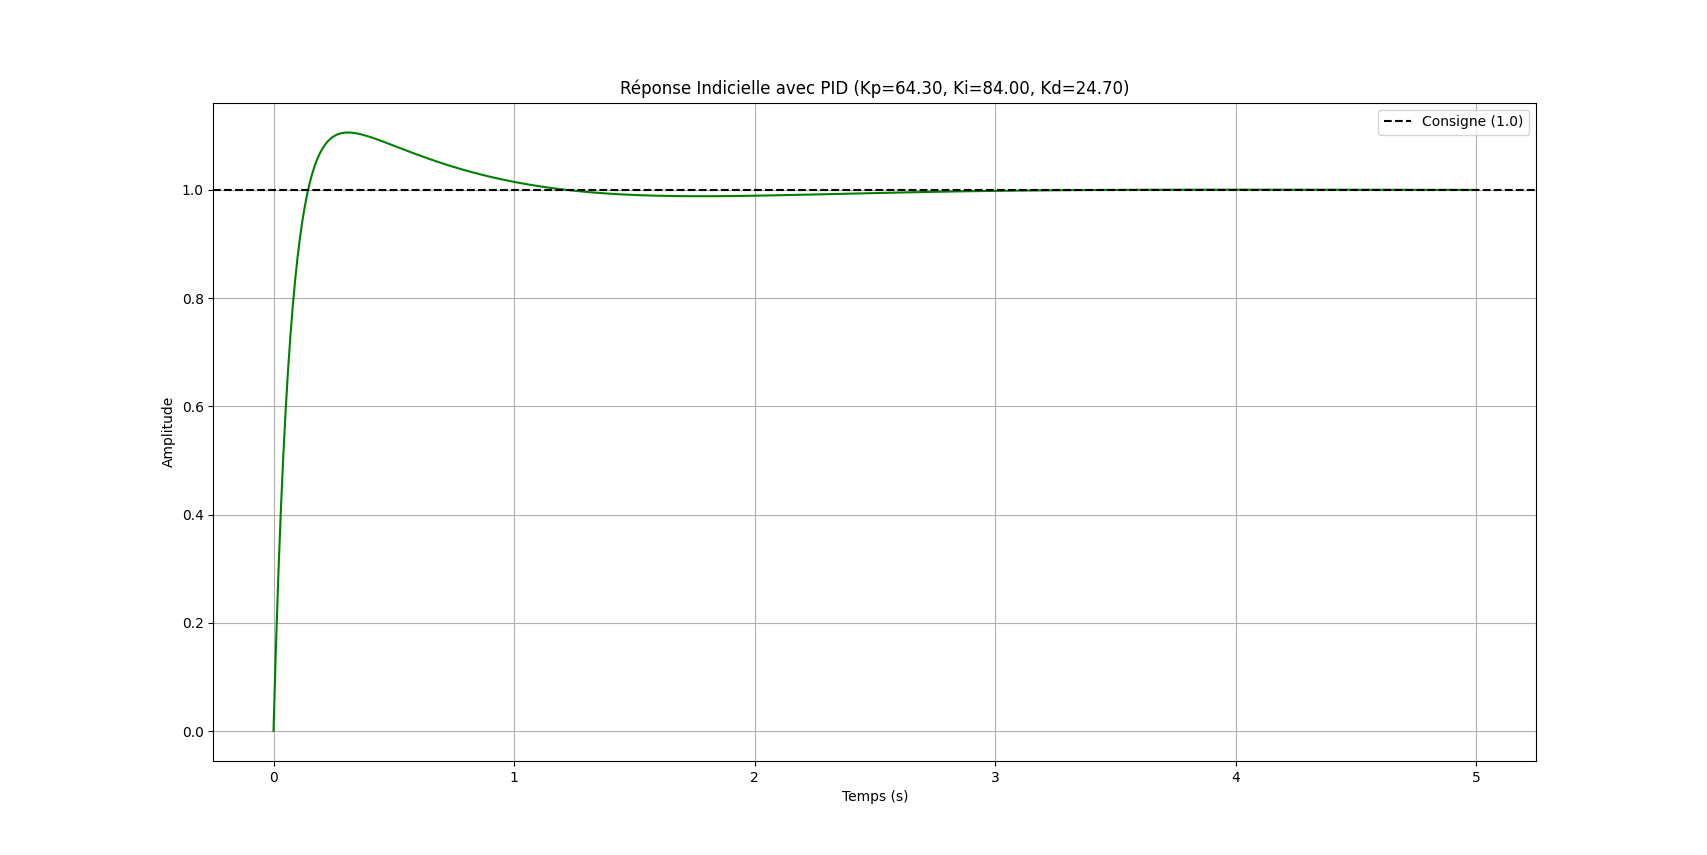
\includegraphics[width=0.9\textwidth]{Figure_5.png}}
    \caption{Réponse indicielle en boucle fermée avec le correcteur PID dimensionné.}
    \label{fig:pid_step}
\end{figure}

\textit{Commentaire :} L'action intégrale élimine complètement l'erreur statique en régime permanent (la valeur converge rigoureusement vers 1.0). De plus, l'ajustement du pôle dominant permet d'obtenir un compromis idéal : le système est devenu extrêmement rapide tout en limitant les oscillations transitoires conformément à l'amortissement cible fixé ($\zeta_d = 0.7$).

\newpage

% --- Section 5 : Conclusion ---
\section{Conclusion}

Ce laboratoire a permis de mettre en application de manière concrète les concepts fondamentaux de l'automatique linéaire continue à l'aide de l'outil informatique Python. L'analyse en boucle ouverte a mis en évidence le caractère fortement oscillatoire et lent du système physique initial en raison de son faible amortissement intrinsèque. 

L'étude de la stabilité via un contrôle proportionnel pur a souligné une parfaite concordance mathématique entre l'approche algébrique de Routh-Hurwitz et les critères graphiques de Nyquist et du lieu des racines, fixant avec précision la limite critique à $K = -0.5$. 

Enfin, la mise en œuvre d'une méthode de synthèse rigoureuse par placement de pôles a permis de dimensionner un correcteur PID performant. Les résultats de la simulation en boucle fermée démontrent la puissance de cette approche, capable de transformer un système initialement instable ou mal amorti en un procédé industriel rapide, précis et doté d'une marge de stabilité parfaitement maîtrisée.

% --- Section 6 : Références ---
\section{Références}

La réalisation de ce laboratoire et la structuration de ce rapport se sont appuyées sur plusieurs ressources théoriques et techniques :

\begin{itemize}
    \item Support et notes du cours d'\textit{Automatique et Robotique}.
    \item Utilisation de l'intelligence artificielle Gemini (Google) pour l'assistance au débogage du code Python et la mise en page du rapport en \LaTeX.
\end{itemize}

\newpage

% --- Section 7 : Annexes ---
\section{Annexes : Code Python complet}

Le script générique utilisé pour générer l'ensemble des résultats numériques et des figures de ce rapport est reproduit ci-dessous :

\begin{verbatim}
import numpy as np
import matplotlib.pyplot as plt
import control as ct
import math
import warnings

# ==============================================================================
# FILTRE D'AVERTISSEMENTS
# ==============================================================================
# Masque les avertissements de dépréciation liés aux mises à jour des librairies
# pour garder une console propre lors de l'exécution.
warnings.filterwarnings("ignore", category=FutureWarning)
warnings.filterwarnings("ignore", category=UserWarning)
warnings.filterwarnings("ignore", category=DeprecationWarning)

# ==============================================================================
# 0. DÉFINITION DE LA FONCTION DE TRANSFERT (Générique)
# ==============================================================================
# Fonction de transfert : H(s) = 2 / (3s^2 + s + 1)
num = [2]
den = [3, 1, 1] 

# Création du système avec la librairie control
H = ct.TransferFunction(num, den)
print("=== FONCTION DE TRANSFERT H(s) ===")
print(H)

# Extraction des coefficients pour les calculs analytiques génériques
N = num[0]
a, b, c = den[0], den[1], den[2]


# ==============================================================================
# 1. CARACTÉRISTIQUES DU SYSTÈME
# ==============================================================================
wn = math.sqrt(c / a)
zeta = b / (2 * math.sqrt(a * c))
K_stat = N / c

print("\n=== CARACTÉRISTIQUES DU SYSTÈME ===")
print(f"Pulsation propre (wn) : {wn:.4f} rad/s")
print(f"Coefficient d'amortissement (zeta) : {zeta:.4f}")
print(f"Gain statique (K) : {K_stat:.4f}")

if zeta < 1:
    print("Analyse : 0 < zeta < 1, le système est sous-amorti (oscillatoire).")
elif zeta == 1:
    print("Analyse : zeta = 1, le système est critique.")
else:
    print("Analyse : zeta > 1, le système est sur-amorti (apériodique).")


# ==============================================================================
# 2 & 3. RÉPONSES IMPULSIONNELLE ET INDICIELLE
# ==============================================================================
t = np.linspace(0, 10, 1000)
t_imp, y_imp = ct.impulse_response(H, t)
t_step, y_step = ct.step_response(H, t)

plt.figure(figsize=(12, 5))

plt.subplot(1, 2, 1)
plt.plot(t_imp, y_imp, color='blue')
plt.title("Réponse Impulsionnelle")
plt.xlabel("Temps (s)")
plt.ylabel("Amplitude")
plt.grid(True)

plt.subplot(1, 2, 2)
plt.plot(t_step, y_step, color='red')
plt.axhline(K_stat, color='black', linestyle='--', label=f'Valeur finale ({K_stat})')
plt.title("Réponse Indicielle (Échelon)")
plt.xlabel("Temps (s)")
plt.ylabel("Amplitude")
plt.legend()
plt.grid(True)

plt.tight_layout()
plt.show()


# ==============================================================================
# 4. COURBES DE BODE
# ==============================================================================
plt.figure()
# Correction : 'margins' est remplacé par 'display_margins'
ct.bode_plot(H, dB=True, display_margins=True)
plt.suptitle("Diagramme de Bode du système en boucle ouverte")
plt.show()


# ==============================================================================
# 5. AMPLITUDE ET PHASE À DES PULSATIONS SPÉCIFIQUES
# ==============================================================================
omegas_test = [0.1, 1, 10]
print("\n=== ANALYSE FRÉQUENTIELLE (Graphique/Automatique vs Analytique) ===")

# Correction : 'freqresp' est remplacé par 'frequency_response'
mag_auto, phase_auto_rad, omega_auto = ct.frequency_response(H, omegas_test)

for i, w in enumerate(omegas_test):
    # --- Automatique ---
    mag_dB_auto = 20 * math.log10(mag_auto[i])
    phase_deg_auto = math.degrees(phase_auto_rad[i])
    
    # --- Analytique ---
    part_re = c - a * (w**2)
    part_im = b * w
    mag_analytique = N / math.sqrt(part_re**2 + part_im**2)
    mag_dB_analytique = 20 * math.log10(mag_analytique)
    phase_rad_analytique = -math.atan2(part_im, part_re)
    phase_deg_analytique = math.degrees(phase_rad_analytique)
    
    print(f"\nPour w = {w} rad/s :")
    print(f"  Automatique -> Amplitude: {mag_dB_auto:.2f} dB, Phase: {phase_deg_auto:.2f}°")
    print(f"  Analytique  -> Amplitude: {mag_dB_analytique:.2f} dB, Phase: {phase_deg_analytique:.2f}°")


# ==============================================================================
# 6. RÉGULATEUR PROPORTIONNEL & CRITÈRE DE NYQUIST (MÉTHODE MANUELLE ROBUSTE)
# ==============================================================================
print("\n=== AJOUT D'UN RÉGULATEUR PROPORTIONNEL (K) ===")
K_limite = -c / N
print(f"Limite de stabilité de K (Critère de Routh) : K > {K_limite}")

K_stable = 1.0          # Cas stable
K_lim = K_limite        # Limite de stabilité
K_instable = -1.0       # Cas instable

cas_K = {'Stable (K=1)': K_stable, 'Limite (K=-0.5)': K_lim, 'Instable (K=-1)': K_instable}

plt.figure(figsize=(15, 5))
# Vecteur de fréquences logarithmique large (de 0.01 à 100 rad/s)
omega_nyq = np.logspace(-2, 2, 2000)

for i, (titre, K) in enumerate(cas_K.items(), 1):
    plt.subplot(1, 3, i)
    
    # 1. Calcul de la réponse en fréquence
    mag, phase, _ = ct.frequency_response(K * H, omega_nyq)
    
    # Sécurité : "aplatir" les tableaux
    mag = np.squeeze(mag)
    phase = np.squeeze(phase)
    
    # 2. Passage en coordonnées cartésiennes (Re, Im)
    Re = mag * np.cos(phase)
    Im = mag * np.sin(phase)
    
    # 3. Tracés propres
    plt.plot(Re, Im, color='blue', label=r'$\omega > 0$')
    plt.plot(Re, -Im, color='red', linestyle='--', label=r'$\omega < 0$')
    
    # 4. Point critique (-1, 0)
    plt.plot(-1, 0, marker='+', color='black', markersize=12, markeredgewidth=2, label='Point critique (-1, 0)')
    
    # Mise en forme du graphique
    plt.title(f"Nyquist : {titre}")
    plt.axhline(0, color='black', linewidth=1) # Axe réel
    plt.axvline(0, color='black', linewidth=1) # Axe imaginaire
    
    # Nouvelles limites plus larges pour ne rien rogner de la résonance
    plt.xlim([-3.5, 3.5])
    plt.ylim([-4.5, 4.5])
    
    plt.grid(True, linestyle=':')
    plt.legend(loc='upper right', fontsize='small')

plt.tight_layout()
plt.show()


# ==============================================================================
# 7. LIEU DES RACINES (Root Locus)
# ==============================================================================
plt.figure()
# Utilisation de la syntaxe standard (les warnings éventuels sont gérés par le filtre)
ct.root_locus(H, plot=True)
plt.title("Lieu des racines (Root Locus)")
plt.show()


# ==============================================================================
# 8. RÉGULATEUR PID (Méthode de Placement de Pôles)
# ==============================================================================
print("\n=== RÉGULATEUR PID (Méthode du Placement de Pôles) ===")
zeta_d = 0.7
wn_d = 2.0
p3 = -10 * zeta_d * wn_d 

Kd = (a * (2 * zeta_d * wn_d - p3) - b) / N
Kp = (a * (wn_d**2 - 2 * zeta_d * wn_d * p3) - c) / N
Ki = (a * (-p3 * wn_d**2)) / N

print("Paramètres calculés pour le PID :")
print(f"Kp = {Kp:.4f}")
print(f"Ki = {Ki:.4f}")
print(f"Kd = {Kd:.4f}")

num_pid = [Kd, Kp, Ki]
den_pid = [1, 0]
C = ct.TransferFunction(num_pid, den_pid)
T_fermee = ct.feedback(C * H, 1)

print("\nFonction de transfert en boucle fermée avec PID :")
print(T_fermee)

t_pid = np.linspace(0, 5, 1000)
t_out, y_out = ct.step_response(T_fermee, t_pid)

plt.figure()
plt.plot(t_out, y_out, color='green')
plt.axhline(1, color='black', linestyle='--', label='Consigne (1.0)')
plt.title(f"Réponse Indicielle avec PID (Kp={Kp:.2f}, Ki={Ki:.2f}, Kd={Kd:.2f})")
plt.xlabel("Temps (s)")
plt.ylabel("Amplitude")
plt.legend()
plt.grid(True)
plt.show()

\end{verbatim}

\end{document}